\documentclass[tikz,border=10pt]{standalone}
\usetikzlibrary{positioning}
\usetikzlibrary{decorations.pathmorphing}
\begin{document}
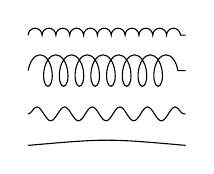
\begin{tikzpicture}
  \draw[decorate,decoration=bumps] (0,0) -- (2,0);
  \draw[decorate,decoration={coil, amplitude=2mm,segment length=2mm},yshift=-4.5mm] (0,0) -- (2,0);
  \draw[decorate,decoration={snake},yshift=-10mm] (0,0) -- (2,0);
  \draw[decorate,decoration={bent},yshift=-14mm] (0,0) -- (2,0);
\end{tikzpicture}
\end{document}
